\section{Fourrier Reihe}
\subsection{Einleitung}
Wir fangen mit einem Beispiel an. Wir wollen uns eine Antenne und vor allem die Ladungsverteilung auf dieser anschauen. Dabei haben wir in einer gewissen Periodität die Ladung verteilt. In unserem ersten Beispiel in Abbildung \ref{fig:antenneladung} jetzt wie eine Sinuskurve:
\begin{figure}[H]
	\begin{tikzpicture}[
			plus/.pic={\draw (-0.1,0)--(0.1,0); \draw(0,-0.1)--(0,0.1);},
			minus/.pic={\draw (-0.1,0) -- (0.1,0);},
		]
		\draw (0,0) rectangle (5,1);
		\path (0.3,0.5)
		\foreach \deltapi in {1,2, ...,9}{
			%\pgfmathrandominteger{\random}{-5}{5}
			++($0.13/(1.1-cos(\deltapi*36)) *(1,0)$)pic {plus}
		}
		\foreach \deltapi in {10,11, ...,19}{
			++($0.10/(1.1-cos(\deltapi*36)) *(1,0)$) pic {minus}
		}
		%\foreach \deltapi in {20,21, ...,29}{
		%	++($0.07/(1.1-cos(\deltapi*36)) *(1,0)$) pic {plus}
		%}
		;

		\begin{scope}[yshift=-1.5cm]
			\draw[->] (0,0) -- (6,0) node[above] {Position};
			\draw[->] (0,-1) -- (0,1) node[left] {Ladung $Q$};
		\shade[x=0.8cm,bottom color=blue, top color=red] (3.14,0) -- (0,0) -- 
			plot file{dat/puresinus1.dat} -- cycle;
		\end{scope}

	\end{tikzpicture} \centering
	\caption{Ladungsverteilung auf Antenne} \label{fig:antenneladung}
\end{figure}
Diese Ladungsverteilung brauchen wir, da wir damit das Elektrodynamische Problem der Signawelle lösen können. Dann könnten wir zum Beispiel bestimmen, wie die Signalstärke von der Richtung abhängig ist.
\begin{figure}[H]
	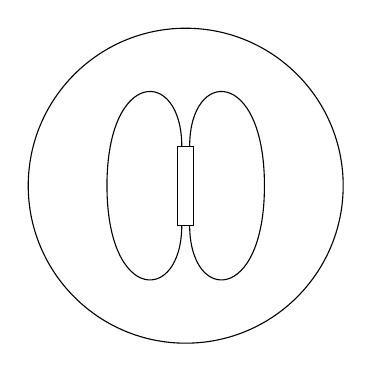
\begin{tikzpicture}[
			antenna/.pic={\draw(-0.1,0.5) rectangle (0.1,-0.5);}
		]
		\pic at(0,0) {antenna};
		\draw (0.05,0.5) .. controls (0.05,1.5) and (1,1.5) .. (1,0) 
			.. controls (1,-1.5) and (0.05,-1.5) .. (0.05,-0.5);
		\draw[xscale=-1] (0.05,0.5) .. controls (0.05,1.5) and (1,1.5) .. (1,0) 
			.. controls (1,-1.5) and (0.05,-1.5) .. (0.05,-0.5);
		\draw (0,0) circle[radius=2cm];
	\end{tikzpicture} \centering
	\caption{Elektrisches Feld um Antenne}
\end{figure}

Da wir die Kurve zur Mathematik bekommen wollen fangen wir jetzt mit Sinuskurven an. Wir denken uns in Abbildung \ref{fig:frequenzaufteilung} ein periodische Ladungsverteilung aus, und spalten diese in verschiedene Sinusfunktionen auf:
\begin{figure}[H]
	\begin{tikzpicture}
		\begin{scope}
			\draw[->] (0,0) -- (9.423,0);
			\draw[->] (0,-2) -- (0,2);
			\draw[smooth] plot file {dat/sinussumme.dat};
			\node(plot1) at (0,0.5) {};
		\end{scope}
		\begin{scope}[yshift=-3.5cm]
			\draw[->] (0,0) -- (9.423,0);
			\draw[->] (0,-1) -- (0,1);
			\draw plot file {dat/sinus1.dat};
			\node(plot2) at (0,0.5) {};
		\end{scope}
		\begin{scope}[yshift=-6cm]
			\draw[->] (0,0) -- (9.423,0);
			\draw[->] (0,-1) -- (0,1);
			\draw plot file {dat/sinus2.dat};
			\node(plot3) at (0,0.5) {};
		\end{scope}
		\draw[->] (plot1) .. controls ($(plot1) + (-1,0)$) and
			($(plot2)+ (-1,0)$) .. (plot2);
		\draw[->] (plot1) .. controls ($(plot1) + (-2,0)$) and
			($(plot3)+ (-2,0)$) .. (plot3);
	\end{tikzpicture}
	\caption{Aufteilung der Ladungsverteilung auf verschieden Frequenzen}\label{fig:frequenzaufteilung}
\end{figure}
Da wir eine periodische Funktion haben können von einem Randproblem ausgehen. Bei jeder Wiederholung startet unsere Verteilung bei $f(n\cdot T) = 0$. Dann können wir davon ausgehen, dass wir unser Problem mit verschiedenen Sinusfunktionen lösen können:
\begin{equation}
	v_i(x) = \sin (i\cdot x f) 
\end{equation}
Da wir die Form unserer Sinusfunktionen nun kennen, brauchen wir nur den Anteil der einzelnen Sinusfunktionen an unserer Verteilung:
\begin{equation}
	f(x) = a_1 v_1(x) + a_2 v_2(x) + \dots
\end{equation}
Interessant ist jetzt nur noch die Amplitude der einzelnen Schwingungen:
\begin{figure}[H]
	\begin{tikzpicture}
		\draw[->] (0,0) -- (1,0);
		\draw[->] (0,0) -- (0,1);
		\draw plot file {dat/sinussumme.dat};
	\end{tikzpicture}
	\caption{Ablesen der Amplituden von den einzelnen Schwingungen} \label{fig:schwingungsaufteilung}
\end{figure}
Nach dieser Aufteilung der Amplituden kann man die Grafik auch als Superpositiion der einzelnen Schwingungen schreiben. Die Grafik \ref{fig:frequenzaufteilung} können wir dadurch als Gleichung aufschreiben.

\subsection{Aufteilung auf die Frequenzen - Tupelform der Verteilung}
Die Verteilung können wir in verschiedene Schwingungen aufteilen:
\begin{equation}
	f(x) = a_1 v_1(x) + a_2 v_2(x) + \dots
\end{equation}
Da wir die Form unserer Schwingungen kennen, brauchen wir für die vollständige Darstellung der Verteilung nur die einzelnen Amplituden. Wir können also die Funktion durch ein Tupel darstellen:
\begin{equation}
	f = \left(a_1, a_2, a_3, \dots \right)
\end{equation}
Das sieht jetzt schon sehr nach einem Vektor aus. Für einen Vektor brauchen wir aber am besten noch ein Skalarprodukt:
\begin{equation}
	a_i = < f | v_i > 
\end{equation}

Mit diesem wollen wir dann auch eine beliebige Verteilung auf einen anderen Vektor abbilden können, wie in unserer Abbildung \ref{fig:vektorprodukt} beispielhaft auf die erste Sinusschwingung(längste Wellenlänge).
\begin{figure}[H]
	\begin{center}
		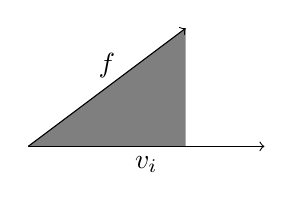
\begin{tikzpicture}
			\draw[->] (0,0) -- (3,0) node[midway, below] {$v_i$};
			\draw[->] (0,0) -- (2,1.5) node[midway, above] {$f$};
			\fill[opacity=0.5] (0,0) -- (2,1.5) -- (2,0) --cycle;
		\end{tikzpicture}
	\end{center}
	\caption{Darstellung des Skalarprodukts in Vektordarstellung}\label{fig:vektorprodukt}
\end{figure}

\subsection{Skalarprodukt stehender Wellen}
Wir brauchen ein Skalarprodukt, dass uns erlaubt eine beliebige Wellenfunktion auf eine Basisschwingung abzubilden. Dafür bedienen wir uns einer der Eigenschaften von Sinusfunktionen.
Wir modulieren dafür verschiedene Schwingungen $v_{2,3,\dots}$ mit einer Schwingung $v_1$. Danach mitteln wir über eine Periode$1/f$.
\begin{equation}
	\int_{1/f}  v_{2,3,\dots} (x) \cdot v_1(x) \mathrm{d}x = 0
\end{equation}
Diese Mittelung ist gleich null, wenn die Frequenz nicht die gleiche ist. bei gleichen Frequenzen erhält man einen Beitrag $\neq 0$.
Wie in Abbildung \ref{fig:schwingungsaufteilung} kann man eine beliebige periodische Funktion auf verschiedene Wellen aufteilen:
\begin{equation}
	f(x) = \sum_i a_i v_i(x)
\end{equation}
Wenn man eine Verteilung wie oben moduliert und danach mittelt, fallen alle Beiträge von Schwingungen die nicht unserer untersuchten Frequenz entsprechen weg:
\begin{eqnarray}
	\int_{1/\nu} f(x) v_1(x) \mathrm{d}x&=\int_{1/\nu} a_1v_1^2(x)  \mathrm{d}x\\
	&=a_1\int_{1/f} v_1^2(x)  \mathrm{d}x
\end{eqnarray}
Wir erhalten also aus dieser Rechnung den Beitrag einer Schwingung $a_1$ an unserer Verteilung $f$. Dies kann man auch mit den anderen Schwingungen $v_i$ durchführen und kann dadurch die anderen Beiträge $a_i$ ermitteln. Außerdem haben wir jetzt eine Rechnungsmethode gefunden die unserem gesuchten Skalarprodukt entspircht:
\begin{equation}
	< f | v_i > =  \frac{1}{\alpha_i}\int_{1/\nu} f(x) v_i(x) \mathrm{d}x
\end{equation}
Dabei brauchen wir auch noch einen Normierungsfaktor $\alpha$:
\begin{equation}
	\alpha_i = <v_i| v_i>
\end{equation}

\subsection{Gewichtungsfaktor bzw Proportionalitätsfaktor}
Beider Mittelung kommt es zu einem Vergrößerungsfaktor $\alpha$. Diesen kann man berechnen indem man den Beitrag einer Welle zu sich selbst berechnet:
\begin{equation}
	< v_i|v_i> = \frac{1}{\alpha} \int \mathrm{sin}^2(x) \mathrm{d}x
\end{equation}

\subsection{Fourrieretransformation - allgemein}
Ursprünglich hatten wir nur bestimmte Schwingungen zugelassen, zB nur sinus-Schwingungen. Wir wollen jetzt zu etwas allgemeineren Formulierungen übergehen und erstmal cosinus-Schwingungen zulassen:
\begin{figure}[H]
	\begin{tikzpicture}[
			sum/.pic={
			\draw[->] (0,0) -- (3.142,0);
			\draw[->] (0,-2) -- (0,2);
			\path[clip] (0,-3) rectangle (3.12,3);
			\draw[smooth] plot file {dat/schwingungsumme.dat};
			\coordinate (-arrowstart) at (0,0.5);
			\coordinate (-bottom left) at (0,-2);
			\coordinate (-bottom right) at (3.142,-2);
			},
			first/.pic={
			\draw[->] (0,0) -- (3.142,0);
			\draw[->] (0,-1.3) -- (0,1.3);
			\path[clip] (0,-2.5) rectangle (3.12,2.5);
			\draw plot file {dat/sinus1.dat};
			\coordinate (-south) at (1.571,-1.3);
			\coordinate (-top right) at (3.142,1.3);
			},
			second/.pic={
			\draw[->] (0,0) -- (3.142,0);
			\draw[->] (0,-1.3) -- (0,1.3);
			\path[clip] (0,-2.5) rectangle (3.12,2.5);
			\draw plot file {dat/sinus2.dat};
			\coordinate (-north) at (1.571,1.3);
			},
			third/.pic={
			\draw[->] (0,0) -- (3.142,0);
			\draw[->] (0,-1.3) -- (0,1.3);
			\path[clip] (0,-2.5) rectangle (3.12,2.5);
			\draw plot file {dat/cosinus1.dat};
			\coordinate (-arrowend) at (0,0.5);
			\coordinate (-south) at (1.571,-1.3);
			\coordinate (-top left) at (0,1.3);
			},
			fourth/.pic={
			\draw[->] (0,0) -- (3.142,0);
			\draw[->] (0,-1.3) -- (0,1.3);
			\path[clip] (0,-2.5) rectangle (3.12,2.5);
			\draw plot file {dat/cosinus2.dat};
			\coordinate (-arrowend) at (0,0.5);
			\coordinate (-north) at (1.571,1.3);
			}
		]
		\path (0,0) pic (picsum) {sum}
		(-2, -3.5) pic (picfirst) {first}
		(-2, -6.5) pic (picsecond) {second}
		(2,-3.5) pic (picthird) {third}
		(2,-6.5) pic (picfourth) {fourth};
		\draw[->] (picsum-arrowstart) 
			.. controls ($(picsum-arrowstart) + (-1,0)$) and
			($(picthird-arrowend)+ (-1,0)$) .. 
			(picthird-arrowend);
		\draw[->] (picsum-arrowstart) 
			.. controls ($(picsum-arrowstart) + (-2,0)$) and
			($(picfourth-arrowend)+ (-2,0)$) .. 
			(picfourth-arrowend);
	\end{tikzpicture} \centering
	\caption{Aufteilung in sinus und cosinus-Schwingungen}
\end{figure}
Da wir keine zwei unterschiedlichen Arten von Basen verwenden wollen, also sinus-Basen $v_i$ und cosinus-Basen $u_i$, wollen wir bei einheitliche zusammenfassen. Dies können wir über die Exponentialfunktion verwirklichen:
\begin{equation}
	\mathrm{exp}(\pm ikx) = \mathrm{cos}(kx) \pm \mathrm{sin}(kx) %
	\label{eq:umrechnungexp}
\end{equation}
Durch den Zusammenhang \ref{eq:umrechnungexp} zwischen exponential-Funktion und den trigonometrischen Funktionen können wir nun uns auf eine Basis nur von Exponentialfunktionen beschränken:
\begin{equation}
	w_n = \mathrm{exp}(ik_nx)
\end{equation}
Hierbei sind allerdings auch negative Wellenvektoren $k$ zugelassen.
\subsection{kontinuirliche Basis}
Als letzten Schritt gehen wir von einer diskreten Basis $w_n$ zu einer kontinuirichen Basis über.
\begin{figure}[H]
	\caption{Übergang von diskreten Basis zu einer kontinuirlichen Basis}
\end{figure}
Wir beschränken uns nun nicht mehr auf einen Index, dem dann Wellenvektoren zugeordnet sind, sondern erlauben alle möglichen Wellenvektoren $k$:
\begin{equation}
	w(k) = \mathrm{exp}(ikx)
\end{equation}
Nun erhalten wir nach der Fourrieretransformation nicht mehr Amplituden einzelner Schwingungen sondern eine Verteilung der Schwingungen:
\begin{equation}
	A(k) = \frac{1}{\alpha} \int f(x) \mathrm{exp}(-ikx) \mathrm{d}x
\end{equation}
Dies führt dazu, dass unsere Ursprungsfunktion $f(x)$ wieder auf eine Funktion $A(k)$ abgebildet wird:
\begin{figure}[H]
	\caption{Abbildung einer Funktion zu ihrer Fourrieretransformierten}
\end{figure}
\subsection{Rücktransformation}

